\paragraph{What the problem is about.} The modern tanh RNN from Problem 2 updates its state as $h_t = \tanh(W x_t + U h_{t-1} + b)$: every step \emph{overwrites} $h$. Nothing in the cell says ``keep what you had''; information only survives if $U$ happens to preserve it, and every step pushes it through a saturating nonlinearity. That is the time-direction analogue of the no-residual transformer in Problem 1, and the Problem 2 diagnostics showed the consequence: the last-token gradient of the modern RNN reaches back 156 and 158 tokens in layers 1--2 but only 10 and 6 tokens in layers 3--4, and the top layers run at 50--70\% tanh saturation.

A GRU adds the missing ``keep'' path. With $z_t=\sigma(W_z x_t+U_z h_{t-1})$ and $r_t=\sigma(W_r x_t+U_r h_{t-1})$,
\[ h_t = (1-z_t)\odot h_{t-1} + z_t\odot \tanh\big(W x_t + U (r_t\odot h_{t-1}) + b\big). \]
Per channel, $z_t$ interpolates between copying the old state and writing a new one, so a channel with $z\approx 0$ is a residual connection through time. The reset gate $r_t$ decides how much of the old state the \emph{candidate} is allowed to see. Everything else (4 layers, depth residuals, pre-norm, MLP after every recurrent layer) is identical to the supplied modern RNN; only $h$ is carried across time.

\paragraph{(a) GRU vs.\ tanh.} Table~\ref{tab:p4} has the numbers. The GRU reaches 3.187 at lr 0.003 and 3.183 at 0.006, against 3.516 for the tuned tanh RNN: a 0.33 improvement, more than the entire spread of the eight Problem-2 interventions (3.48--3.58) and bigger than I predicted (locked prediction: $\geq 0.10$). The best rate is also higher (0.003--0.006 vs.\ 0.001--0.002 for the tanh variants), which fits the mechanism: the keep path makes the recurrence contractive by construction, so the cell tolerates larger steps without the recurrent Jacobian blowing up.

\begin{table}[H]\centering\small
\caption{P4, recurrent cells (4 layers, same depth residuals, pre-norm and MLPs as the modern RNN): final validation loss.}\label{tab:p4}
\begin{tabular}{lrrrr}\toprule
variant & lr 0.0015 & lr 0.003 & lr 0.006 & best $-$ additive \\\midrule
modern tanh RNN (supplied) & -- & -- & -- & 3.5160 \\
GRU & 3.2312 & 3.1874 & 3.1829 & -0.3331 \\
GRU, no reset gate & -- & 3.2846 & -- & -0.2314 \\
GRU, reset gate only & -- & 3.4040 & -- & -0.1120 \\
GRU, input-only update gate & -- & 3.2203 & -- & -0.2957 \\
NormGate (ours) & 3.3764 & 3.3768 & -- & -0.1396 \\
NormGate, zero update bias & -- & 3.3533 & -- & -0.1627 \\
\bottomrule\end{tabular}\end{table}

\paragraph{(b) Which part of the GRU matters.} Three ablations, each at lr 0.003, each removing one ingredient:
\begin{itemize}\setlength\itemsep{0pt}
\item \textbf{no reset gate} ($r\equiv 1$): the candidate always sees the whole old state. Tests whether $r$ does anything beyond what $z$ already does.
\item \textbf{reset gate only} ($z\equiv 1$): a tanh RNN whose recurrent input is gated, but with no keep path. If the keep path is the point, this should land near the tanh baseline.
\item \textbf{input-only update gate} ($z_t=\sigma(W_z x_t)$): the cell still has a keep path, but the decision to keep or write cannot look at the state. Tests how much the \emph{content-dependence} of the gate is worth.
\end{itemize}
Locked prediction: update gate $\gg$ reset gate; reset-only ends within 0.05 of tanh; input-only gating loses a few hundredths.
Three ablations at lr 0.003, each removing one piece of the GRU (Table~\ref{tab:p4}):

\begin{enumerate}[nosep]
\item \textbf{No reset gate} ($r_t\equiv 1$): 3.285, i.e.\ 0.10 worse than the full GRU but still 0.23 better than tanh.
\item \textbf{Reset gate only} ($z_t\equiv 1$, no keep path): 3.404, 0.22 worse than the GRU, 0.11 better than tanh.
\item \textbf{Input-only update gate} ($z_t=\sigma(W_z x_t)$, no $U_z h_{t-1}$ term): 3.220, only 0.033 worse than the full GRU. The update gate barely needs to look at the state: deciding ``how much to overwrite'' from the current token alone recovers 90\% of the GRU's gain, which fits the picture of $z_t$ as a per-token write-strength knob rather than a content-based memory controller.
\end{enumerate}

Reading the table: the keep path $(1-z_t)\odot h_{t-1}$ is the big piece (removing it costs 0.22), the reset gate is the smaller piece (0.10), and they are not independent, since the sum of the two costs (0.32) is about the whole GRU-minus-tanh gap (0.33). The order matches my prediction; the size of the reset-gate cost does not. I expected reset-only to be within 0.05 of tanh, and it is 0.11 better, so a gate that only decides how much of the old state the candidate may read already buys a third of the GRU's gain. The reason, in hindsight: the tanh cell's problem is not just that it overwrites $h$, it is that the recurrent input $Uh_{t-1}$ is whatever scale $h$ happens to have, so the candidate saturates (Problem 2 measured 52\% of top-layer units at $|h|>0.95$). A reset gate can shrink that input to zero whenever it would saturate; the keep path cannot do that by itself.


\paragraph{(c) Diagnostics.} Table~\ref{tab:p4diag} and Figure~\ref{fig:p4time} are the same three probes as in Problem 2 (FP32, gradients on, 8 validation sequences, final checkpoints at lr 0.003): how far back the last-token gradient reaches (steps back until it falls to $10^{-3}$ of its value at the last position), the hidden-state RMS, and the fraction of saturated units $\Pr(|h|>0.95)$.

\begin{table}[H]\centering\small
\caption{P4 temporal diagnostics on the final checkpoints (lr 0.003). Reach is per layer (bottom to top); a reach of 1023 means the gradient never fell below $10^{-3}$ of its final value anywhere in the 1024-token window. Saturation is the mean over positions of $\Pr(|h|>0.95)$, per layer.}\label{tab:p4diag}
\begin{tabular}{lrll}\toprule
cell & loss & last-token gradient reach & saturation \\\midrule
modern tanh RNN (supplied) & 3.516 & [156, 158, 10, 6] & [0.15, 0.26, 0.68, 0.52] \\
GRU & 3.187 & [407, 1023, 1023, 1023] & [0.00, 0.01, 0.01, 0.01] \\
GRU, no reset gate & 3.285 & [524, 1023, 1023, 1023] & [0.00, 0.11, 0.69, 0.80] \\
GRU, reset gate only & 3.404 & [164, 217, 214, 109] & [0.16, 0.00, 0.01, 0.03] \\
GRU, input-only update gate & 3.220 & [473, 1023, 1023, 1023] & [0.00, 0.02, 0.08, 0.11] \\
NormGate (ours) & 3.377 & [1023, 1023, 1023, 1023] & [0.18, 0.83, 0.94, 0.94] \\
NormGate, zero update bias & 3.353 & [1023, 1023, 1023, 1023] & [0.11, 0.75, 0.94, 0.93] \\
\bottomrule\end{tabular}\end{table}

\begin{figure}[H]\centering
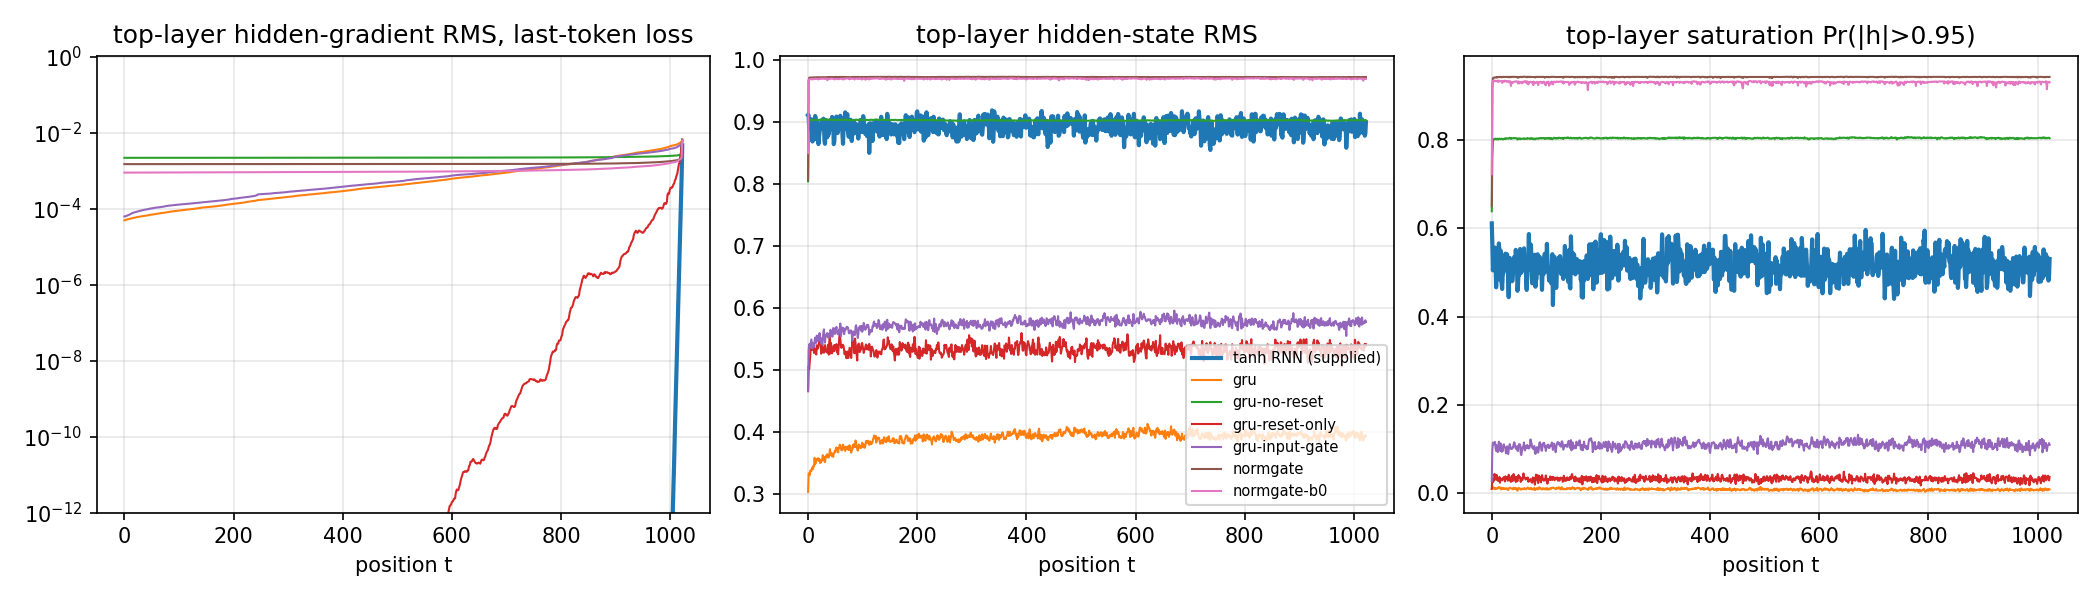
\includegraphics[width=\textwidth]{p4_time.png}
\caption{Top-layer temporal diagnostics vs.\ position for the P4 cells (final checkpoints, lr 0.003). Left: hidden-gradient RMS from the last-token loss (log scale; a flat line means the gradient reaches the whole window). Middle: hidden-state RMS. Right: saturation $\Pr(|h|>0.95)$.}\label{fig:p4time}
\end{figure}

Three things the table says, in order of how much they surprised me.

\textbf{The update gate fixes gradient reach completely.} Every cell with a keep path $(1-z_t)\odot h_{t-1}$ (GRU, no-reset, input-only, both NormGates) has a flat last-token gradient across the entire 1024-token window in layers 2--4: the gradient simply never decays (Figure~\ref{fig:p4time}, left). The tanh RNN's reach was 6--10 steps in the top two layers. This is the ``highway through time'' that the gate provides: with $z_t$ small, $\partial h_t/\partial h_{t-1}\approx(1-z_t)\,I$, so the Jacobian product does not shrink. The reset-only cell, which has no keep path, is the exception: reach 109--217, and its gradient falls off even faster than the tanh RNN's (it is overwriting the state every step, so credit cannot travel). Yet reset-only still beats tanh by 0.11, so reach is not the only thing that matters.

\textbf{The GRU keeps its state small and unsaturated; the tanh RNN cannot.} The GRU's top-layer hidden RMS is 0.40 with 1\% of units saturated, versus 0.90 and 52\% for the tanh RNN. The reset gate is what buys this: remove it (no-reset) and the top two layers saturate to 69--80\%, with RMS back at 0.90, and the loss gives up 0.10. The reset gate's job in this model is to stop the candidate from feeding the full old state back into the $\tanh$, which is exactly the positive-feedback loop that drives a plain tanh RNN to $\pm1$. This is why my prediction in (b) that the reset gate would be the cheap part was wrong: it is the anti-saturation mechanism, and saturation is the modern RNN's main disease (Problem 2).

\textbf{Gradient reach and useful information are different things.} NormGate has the longest reach in the table (1023 in every layer) and still loses to the GRU by 0.19, because 94\% of its top-layer units sit at $|h|>0.95$: the state is a near-binary vector. Normalizing to unit RMS before the candidate makes the candidate's $\tanh$ receive $O(1)$ inputs every step, so it saturates, and the gate then faithfully carries a saturated state forward with perfect gradient flow. A gradient that reaches 1000 steps back through a state that can only hold a sign per unit is not worth much. The GRU's recipe, small state with the resolution of a float, is the better one; the reset-only cell, which has short reach but low saturation (3\%), is the mirror image, and it beats NormGate by only 0.03 despite a 10$\times$ shorter reach. Reach is necessary for long-range credit; it is not sufficient for a good state.

\paragraph{(d) My update: NormGate.} Design, fixed before training: keep the GRU's update gate, drop the reset gate (per (b) it should be the cheap part), normalize the state before it enters the candidate, and bias the gate towards keeping:
\[ h_t = (1-z_t)\odot h_{t-1} + z_t\odot\tanh\big(W x_t + U\,\mathrm{RMSNorm}(h_{t-1}) + b\big),\qquad z_t=\sigma(W_z x_t+U_z h_{t-1} - 1). \]
The RMSNorm attacks the saturation problem directly: the candidate's recurrent input has unit scale no matter how large $h$ has grown, so $\tanh$ stays in its linear range longer. The $-1$ bias starts every channel at $z\approx 0.27$ (keep 73\%), the usual trick for long memory at initialization. A control with the bias at 0 separates the two ideas. Still only $h$ crosses time steps.
\textbf{Result: NormGate reaches 3.376 at both lr 0.0015 and 0.003 (Table~\ref{tab:p4}), 0.14 better than the tanh RNN and 0.19 worse than the GRU.} My prediction (within 0.02 of the GRU) was wrong by an order of magnitude. The bias control settles where the damage came from: with a zero update-gate bias the same cell gets 3.353, so the ``start by keeping'' bias cost 0.023 rather than helping, and the remaining 0.17 gap to the GRU is the normalization itself. The diagnostics in (c) show what the normalization did: it saturated 94\% of the top-layer units, so the cell had perfect gradient reach into a state that had lost its resolution.

Why normalizing the state hurts, given that saturation was the diagnosed problem: RMSNorm removes the state's \emph{scale}, and the scale is information. In a GRU, a unit that has been written many times without being overwritten grows in magnitude and saturates the candidate's $\tanh$, which effectively freezes it; that is a crude but useful ``this slot is full'' signal. NormGate rescales every slot to unit RMS before the candidate reads it, so a slot that holds a confident, long-lived value looks the same as one holding noise, and the candidate cannot tell which to protect. The no-reset GRU (3.285), which also lacks the reset path but keeps the raw state, is 0.09 better than NormGate: the normalization alone costs about that much. The flat lr response (identical losses at 0.0015 and 0.003) is the one thing the normalization did buy: a wider stable learning-rate range, bought at a price in loss.
